% !TeX encoding = UTF-8
% !TeX spellcheck = es_ES

\documentclass[25pt,a0paper,portrait]{tikzposter}
\usepackage[spanish]{babel}
\usepackage[utf8]{inputenc}
%\usepackage[T1]{fontenc}
%\usepackage{lmodern}
\usepackage[super]{nth}
\usepackage{graphicx}
\usepackage[affil-it]{authblk}
% \usepackage{lmodern}
\usepackage{etoolbox}
\usepackage{amsmath}
\usepackage{amssymb}
\usepackage{mathtools}
\renewcommand\Authfont{\LARGE}
\renewcommand\Affilfont{\Large\itshape}

\newlength\htblockbox
\newcommand{\mtblock}[3]{%
\block{#2}{%
\setlength{\htblockbox}{#1}%
\parbox[t][\htblockbox][c]{\linewidth}{#3}}}

\usetheme{Simple}
%\usetitlestyle{verticalShading}


\title{\parbox{\linewidth}{\centering drexml: una herramienta para el descubrimiento de dianas terapéuticas en Enfermeddad Raras}}

\author[1,2]{\large Marina Esteban-Medina}
\author[1,2]{\large V\'ictor Manuel de la Oliva Roque}
\author[3,4,5,6]{\large Sara Herr\'aiz-Gil}
\author[7,1]{\large Mar\'ia Pe\~na-Chilet}
\author[1,2,8,9]{\large Joaqu\'in Dopazo}
\author[1,2,8]{\large Carlos Loucera}

\affil[1]{%
\large Platform for Computational Medicine, Andalusian Public Foundation Progress and Health-FPS, Seville, Spain}

\affil[2]{%
\large Computational Systems Medicine, Institute of Biomedicine of Seville (IBIS), Hospital Virgen del Roc\'io, Seville, Spain}

\affil[3]{%
\large Centro de Investigaci\'on Biom\'edica en Red de Enfermedades Raras (CIBERER-ISCIII), U714, Madrid, Spain}

\affil[4]{%
\large Departamento de Bioingenier\'ia, Universidad Carlos III de Madrid (UC3M), Madrid, Spain}

\affil[5]{%
\large Regenerative Medicine and Tissue Engineering Group, Instituto de Investigaci\'on Sanitaria-Fundaci\'on Jim\'enez D\'iaz University Hospital (IIS-FJD), Madrid, Spain}

\affil[6]{%
\large Epithelial Biomedicine Division, Centro de Investigaciones Energ\'eticas, Medioambientales y Tecnol\'ogicas (CIEMAT), Madrid, Spain}

\affil[7]{%
\large Platform of Big Data, AI and Biostatistics. Health Research Institute La Fe (IISLAFE). Valencia. Spain
}

\affil[8]{%
\large Centro de Investigaci\'on Biom\'edica en Red de Enfermedades Raras (CIBERER-ISCIII), U715, Seville, Spain}

\affil[9]{%
\large FPS/ELIXIR-es, Hospital Virgen del Roc\'io, Seville, Spain}

\institute{\Large{\bf\textsc{XVII Reunión anual CIBERER (2024)}}}

%Make title customizer
\makeatletter
\def\maketitle{\AB@maketitle}
\makeatother

%% Optional title graphic
%\titlegraphic{\includegraphics[width=7cm]{IMG_1934}}
%% Uncomment to switch off tikzposter footer
\tikzposterlatexaffectionproofoff

\begin{document}
\maketitle[width=\linewidth,titletotopverticalspace=-0.05cm]

\block{Introducción}{
    Drexml es una herramienta de software que utiliza aprendizaje automático para identificar nuevos usos para medicamentos existentes. Se ha validado con éxito en dos enfermedades raras: anemia de Fanconi y melanoma familiar. El modelo identifica dianas terapéuticas para enfermedades específicas mediante el empleo de aprendizaje automático y modelado mecanicista de la transducción de señales. En el caso de la anemia de Fanconi, el modelo predice con éxito fármacos reutilizados previamente validados, mientras que en el caso del melanoma familiar, identifica un conjunto prometedor de fármacos para futuras investigaciones.
}

% \note[rotate=8, connection, width = 7cm,
% % roundedcorners=15, targetoffsetx=2cm
% ]{Oh wait! A note!}

\begin{columns}

    \column{0.33}
        \block{\textsc{(a0)} Mapa de la enfermedad}{
            \begin{itemize}
            \item Genes en Orphanet, DisGeNet, \dots?
            \item Control Vs Case?
            \item Pathways?.
            \end{itemize}
        }

    \column{0.33}
        \block{\textsc{(a1)} Transducción de la Señal}{
            \[
                S_{n} = v_{n} \left(1 - \prod_{s_{a} \in A} \left( 1 - s_{a} \right) \right) \prod_{s_{i} \in I} \left( 1- s_{i} \right)
            \]
        }

    \column{0.34}
        \block{\textsc{(a2)} Contextualizar dianas}{
            \[
                \phi_i^k = \frac{1}{K!} \sum_{S \subseteq F \backslash\{i\}} \frac{|S|!(n_{circuits}-|S|-1)!}{n_{circuits}!} [f_x(S \cup \{i\}) - f_x(S)]   
            \]
        }

\end{columns}

\begin{columns}
    \column{0.33}
        \block{\textsc{(a3)} MultiTask Machine Learning}{%
            Can {\bf\textsc{Map Activity}} be predicted from (Drugbank) {\bf\textsc{KDT}}?
            Can we infer what KDT are important to regulate the map. 
            \textit{Learn}  KDT-Signalization \textit{relationships}.
        }
        \block{\textsc{(a4)} Model Explanations}{%
            \begin{itemize}
                \item Useful but too broad.
                \item They (only) speak us about the whole map.
            \end{itemize}
        }
        \block{\textsc{(a5)} SHapley Additive exPlanations}{%
            \begin{itemize}
                \item Fair feature and sample wise contributions.
                \item Disaggregated by circuit by construction.
                \item Additive (aggregated by biologically-relevant groups)
            \end{itemize}
        }
        \block{\textsc{(a6)} Validación basada en Datos}{%
            \begin{itemize}
                \item Optimization + Performance with Repeated Nested CV
                \item Explainability tested with novel methods (Nogueira)
            \end{itemize}
        }
    \column{0.67}
        \block{A Modular Methodology}{%
            \begin{tikzfigure}
            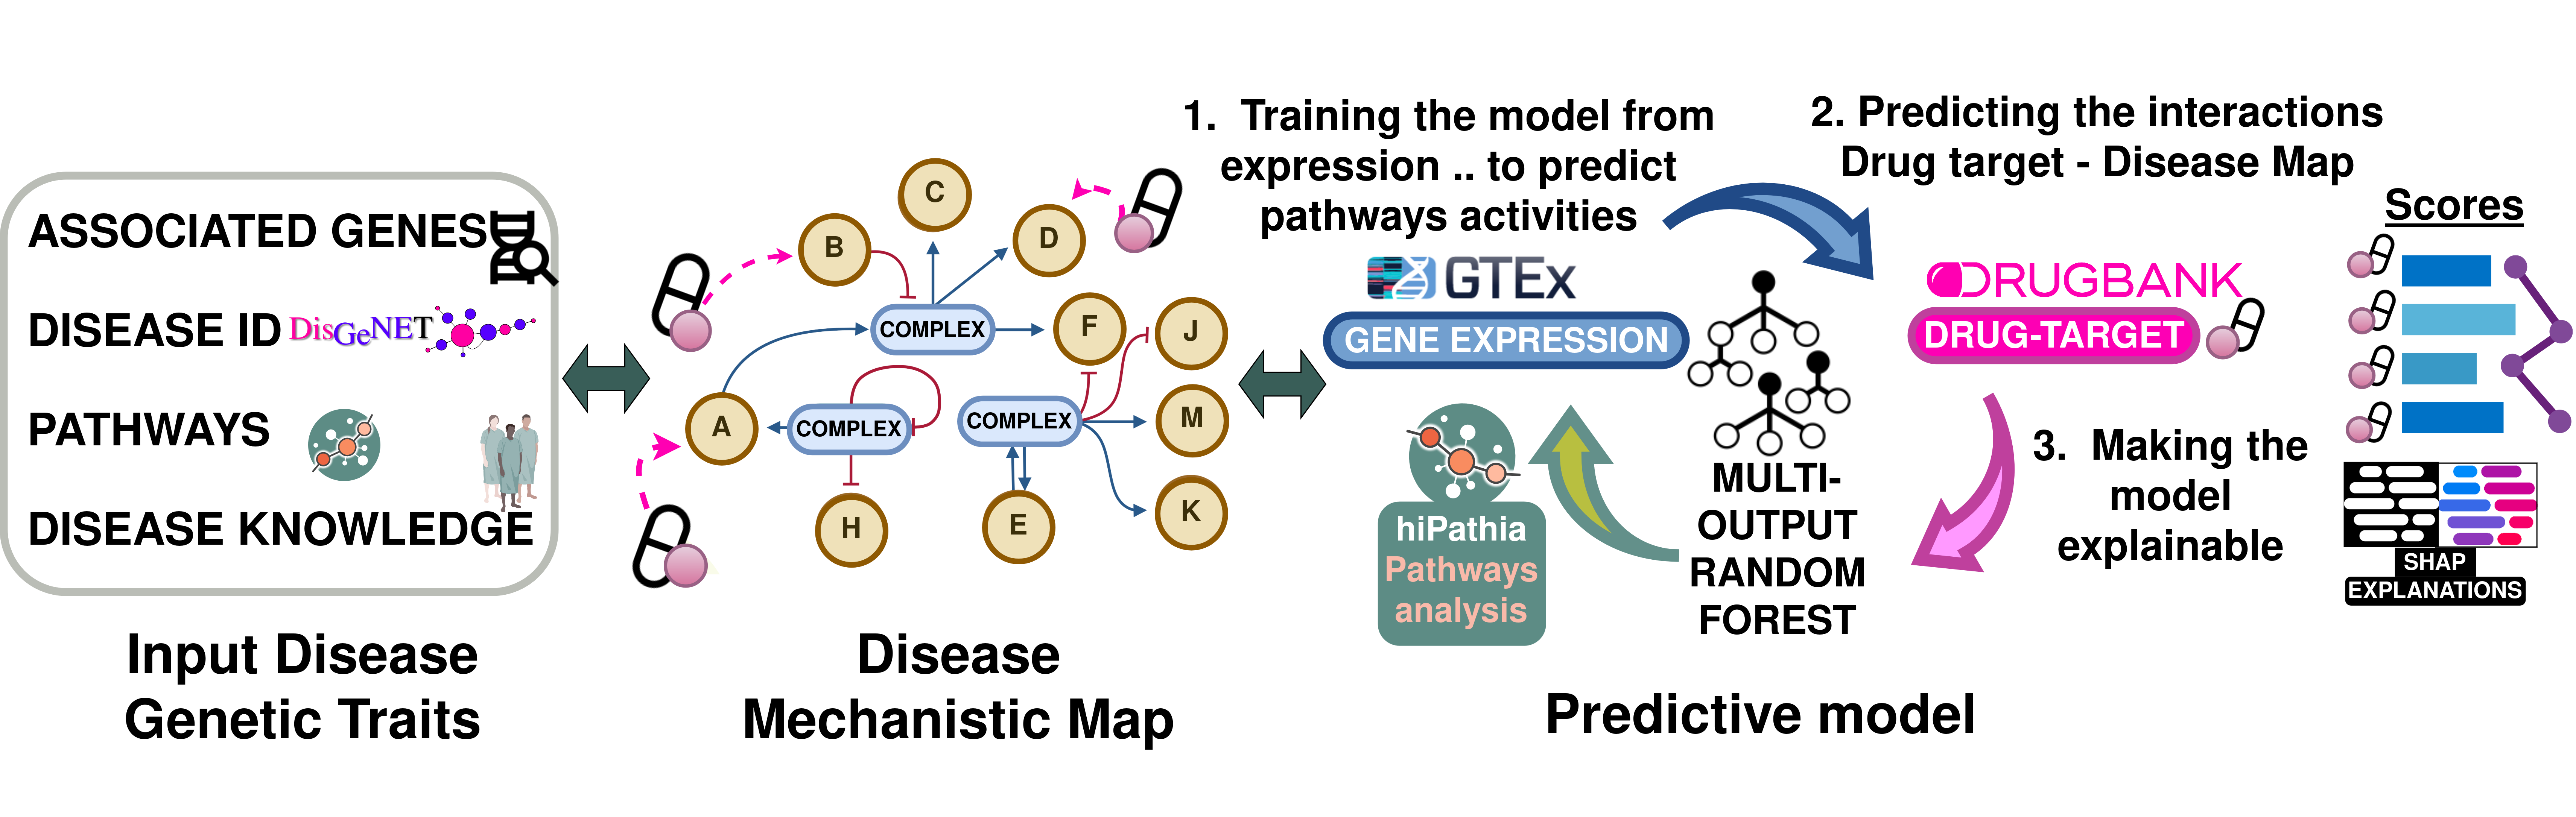
\includegraphics[width=\linewidth]{./fig/drexml/drexml_font_L.png}
            \end{tikzfigure}
        }

        % \note[rotate=8, connection=true, width = 7cm,
        % targetoffsetx=-6cm,targetoffsety=8cm
        % % roundedcorners=15, targetoffsetx=2cm
        % ]{Oh wait! A note!}
\end{columns}

\begin{columns}
    \column{0.6}
    \block{\textsc{(b, c)} Findings}{
        \begin{itemize}
            \item 380 KDTs (targeted by 679 drugs) have direct influence over the whole or partial parts of the map.
            
            \item The GO biological processes enriched are mostly related to immune activity (T-cell, inflammatory response)
            
            \item The COVID-19 Hallmarks are represented.
            
        \end{itemize}
    }
    \column{0.4}
    \block{Trabajos futuros}{%
        \begin{itemize}
            \item Speed the computation (GPU extensions).
            
            \item Develop \textit{sign} like \textsc{SHAP} aggregations.
            
            \item Aggregations in \textit{task}-space.

        \end{itemize}
    }
\end{columns}

\begin{columns}

    \column{0.5}
        \mtblock{2cm}{Funding}{%
            \raisebox{-0.5\height}{\includegraphics[width=0.3\linewidth]{./fig/bbva.pdf}}
            \hspace{\stretch{1}}
            \raisebox{-0.5\height}{
\includegraphics[width=0.3\linewidth]{./fig/ministerio.pdf}}
            \hspace{\stretch{1}}
            \raisebox{-0.5\height}{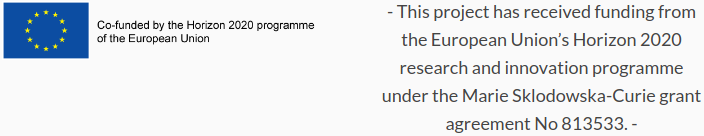
\includegraphics[width=0.3\linewidth]{./fig/mlfpm_grant.png}}
        }

    \column{0.5}
        \mtblock{2cm}{Speaker Affiliations}{%
            \raisebox{-0.5\height}{\includegraphics[width=0.08\linewidth]{./fig/cab_logo_vectorizado.pdf}}
            \hspace{\stretch{1}}
            \raisebox{-0.5\height}{\includegraphics[width=0.44\linewidth]{./fig/FPS_Con_pastilla.jpg}}
            \hspace{\stretch{1}}
            \raisebox{-0.5\height}{
\includegraphics[width=0.22\linewidth]{./fig/ibis_logo.png}}
        }

\end{columns}

\end{document}